\documentclass[utf8, xcolor, usenames,dvipsnames, aspectratio=169, notes, ]{beamer}
\usepackage[german] {babel}
\usepackage[T1]{fontenc}

\usepackage{amsmath, amsfonts, graphicx}
\usepackage{bibunits, tikz}
\usepackage{multirow}
\usepackage{float}
	
	\usepackage{color, colortbl}


\usetheme{progressbar}

\setbeamersize
  {text margin left=4em, text margin right=1em}

\title
  [Vertragsverwaltungs-Prozess]{Einführung eines Vertragsverwaltungs-Prozesses \centering bei der codecentric AG}
  
  \subtitle{(Introduction of a Contract Management Workflow
  	at codecentric AG)}

\author
  [Pia Erbrath]
  {Pia Erbrath (2300869)}

\date
  {Venlo, \today}

\institute
  {FHTenL Venlo}

\begin{document}

\maketitle

\begin{frame}{Übersicht}

  \tableofcontents

\end{frame}

\section{Aufgabe}
\begin{frame}{Aufgabe}
	\begin{itemize}
		\item Kunde: codecentric AG
		\item Einführung der elektronischen Unterschrift als unternehmensweiten Standard
		\item Automatisierung \& Digitalisierung des Unterschreibungsprozesses \newline mit Standardsystemen 
	\end{itemize}
\end{frame}
%\note{ha}

\section{Analyse der initialen Situation}
\begin{frame}{Businessprozess}
	\begin{figure}
		\centering
		\colorbox{white}{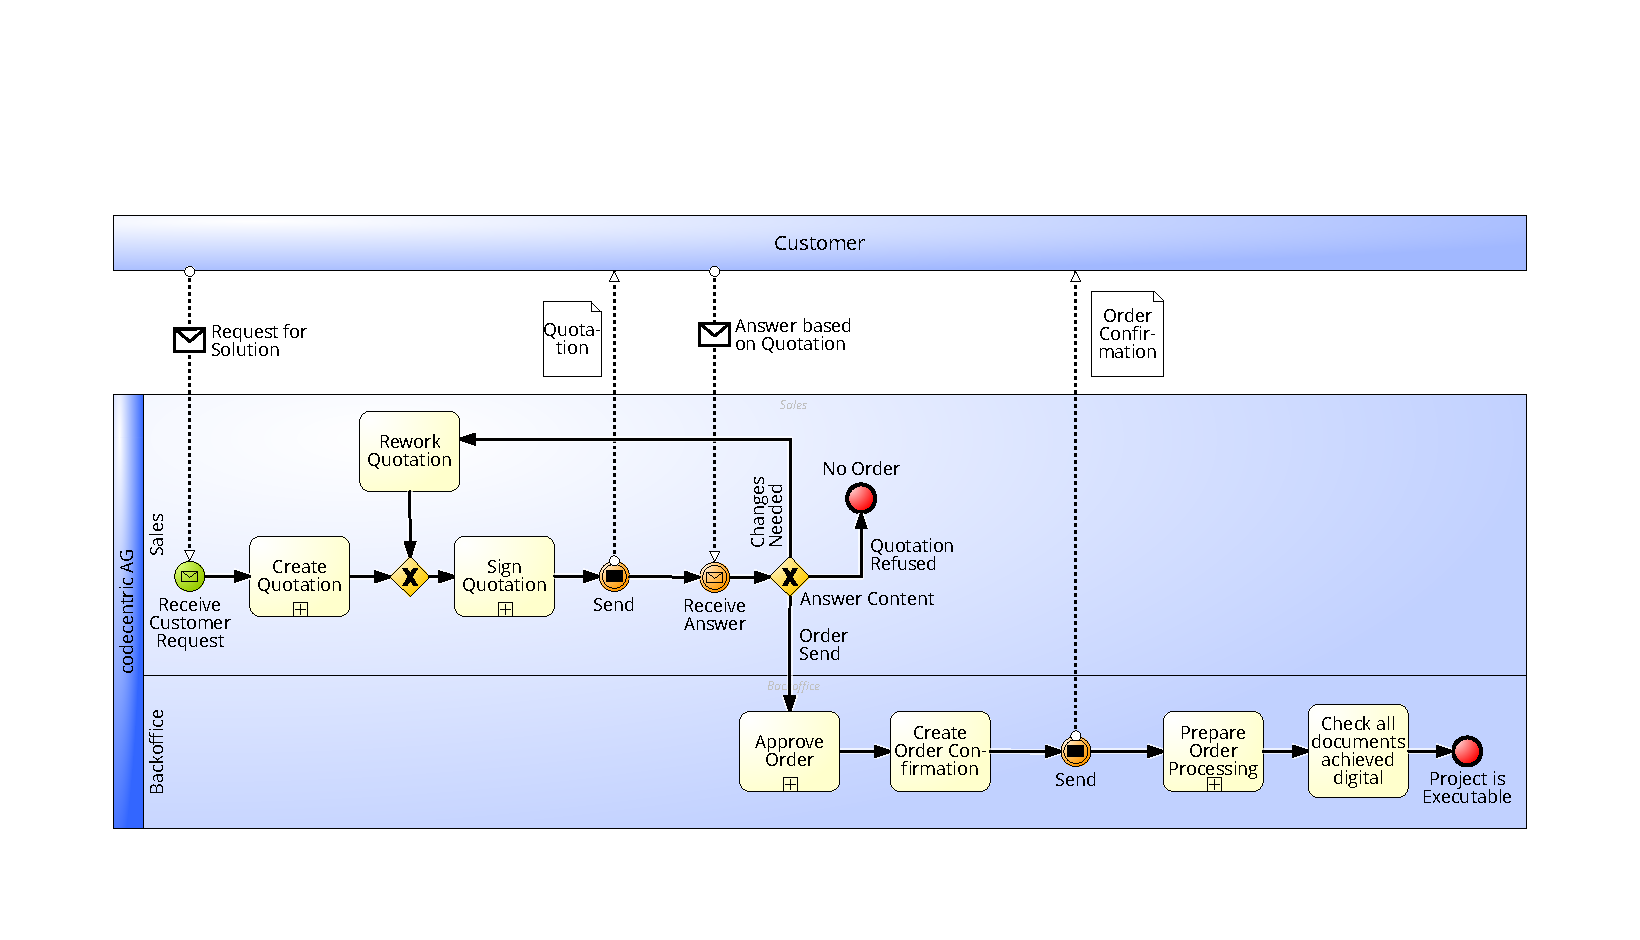
\includegraphics[width=0.93\textwidth, height=0.78\textheight]{./images/0_main}}
	\end{figure}
\end{frame}
%\note{Gut durchführen!!!}

\begin{frame}{Probleme}
	\begin{itemize}
		\item Zu hoher manueller Aufwand	
		\item Inkorrekt unterzeichnete Dokumente 
		\begin{itemize}
			\item Fehlende Unterschrift
			\item Falscher / fehlender Unterzeichner
		\end{itemize}
		\item Veraltete Unterschriftenrichtlinie
		\item Dokumentenerstellung
	\end{itemize}
\end{frame}

\section{Bedingungen an den neuen Prozess \& das System}
\begin{frame}{Ziele}
	\begin{itemize}
		\item Erarbeitet und Abgeklärt mit Beteiligten
	\end{itemize}
	\begin{enumerate}
		\item Erfüllung der aktuellsten Unterschriftenrichlinie
		\item Reduzierung des manuellen Aufwandes
		\item Reduzierung der Papiernutzung
		\item Einheitliches Dokumentenlayout
	\end{enumerate}
\end{frame}

\begin{frame}{Bedingungen}
	\begin{itemize}
		\item Standardprozesse (Automatisierung, vorgegebene Handlungsschritte)
		\item Transparenz \& Prüfung der Unterschriftenrichtlinie
		\item Rechtskonformität
		\item Akzeptanz von verschiedenen Dokumentformaten
	\end{itemize}
\end{frame}

\section{Recherche zum Tool für die elektronische Unterschrift}

\begin{frame}{Kriterien}
	\begin{itemize}
		\item Kriterien gefunden, definiert, gewichtet \& abgeklärt mit Beteiligten
		\item Insgesamt 8 (Auszug):
		\begin{itemize}
			\item Integrationsmöglichkeit
			\item Hard-/Software unabhängig
			\item Handhabung
			\item Kosten
		\end{itemize}
		\item Testszenario mit Protokollen
	\end{itemize}
\end{frame}

\begin{frame}{Ergebnis}
	\newcolumntype{g}{>{\columncolor{bgLightGreen}}c}
	\begin{itemize}
		\item Auswahl: Internetrecherche, Empfehlungen \& Kontakte Mitarbeitern 
		\item Insgesamt 9 Tools
	\end{itemize}
	\pause
	\begin{table}	
	\colorbox{white}{\begin{tabular}{|l|c|g|c|} \hline
		\textbf{Kriterium} & \textbf{SignNow} & \textbf{DocuSign} & \textbf{eSignAnyWhere} \\ \hline
		Integration & + + & + + & + \\ \hline
		Unabhängigkeit & + + & + + & + + \\ \hline
		Handhabung & o & + & + \\ \hline
		Kosten & + + & + & + + \\ \hline
		Sieger & 1 & 2 & 3 \\ \hline
	\end{tabular}}
	\centering
	\caption{Auswahl der Tools und Kriterien}
	\end{table}
\end{frame}


\section{System Design}
\begin{frame}{Generelles Design}
	\begin{figure}[t]
		\centering
		\colorbox{white}{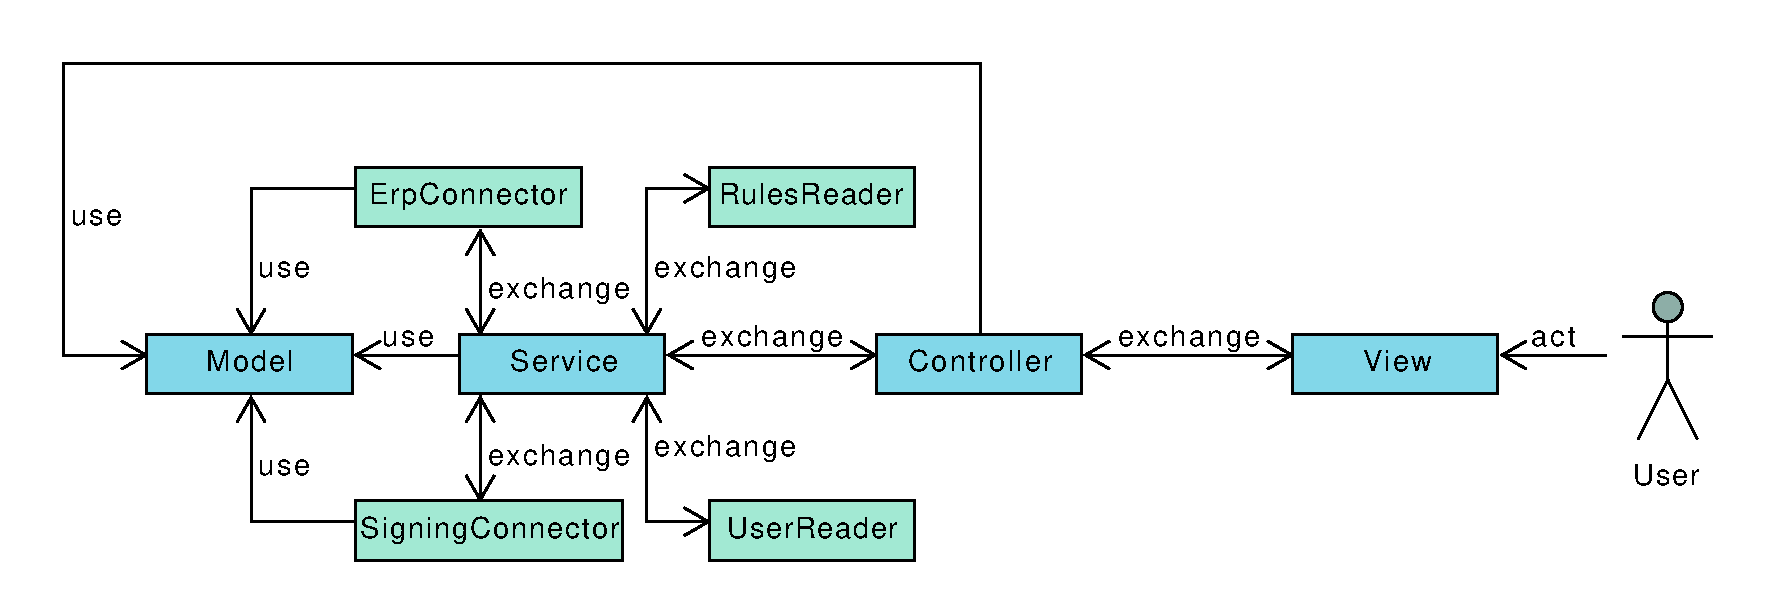
\includegraphics[width=0.9\textwidth, height=0.65\textheight]{./images/generalCommunication.pdf}}
	\end{figure}
\end{frame}

\begin{frame}{Anfrage Unterschriften Gruppen}
	\begin{figure}
		\centering
		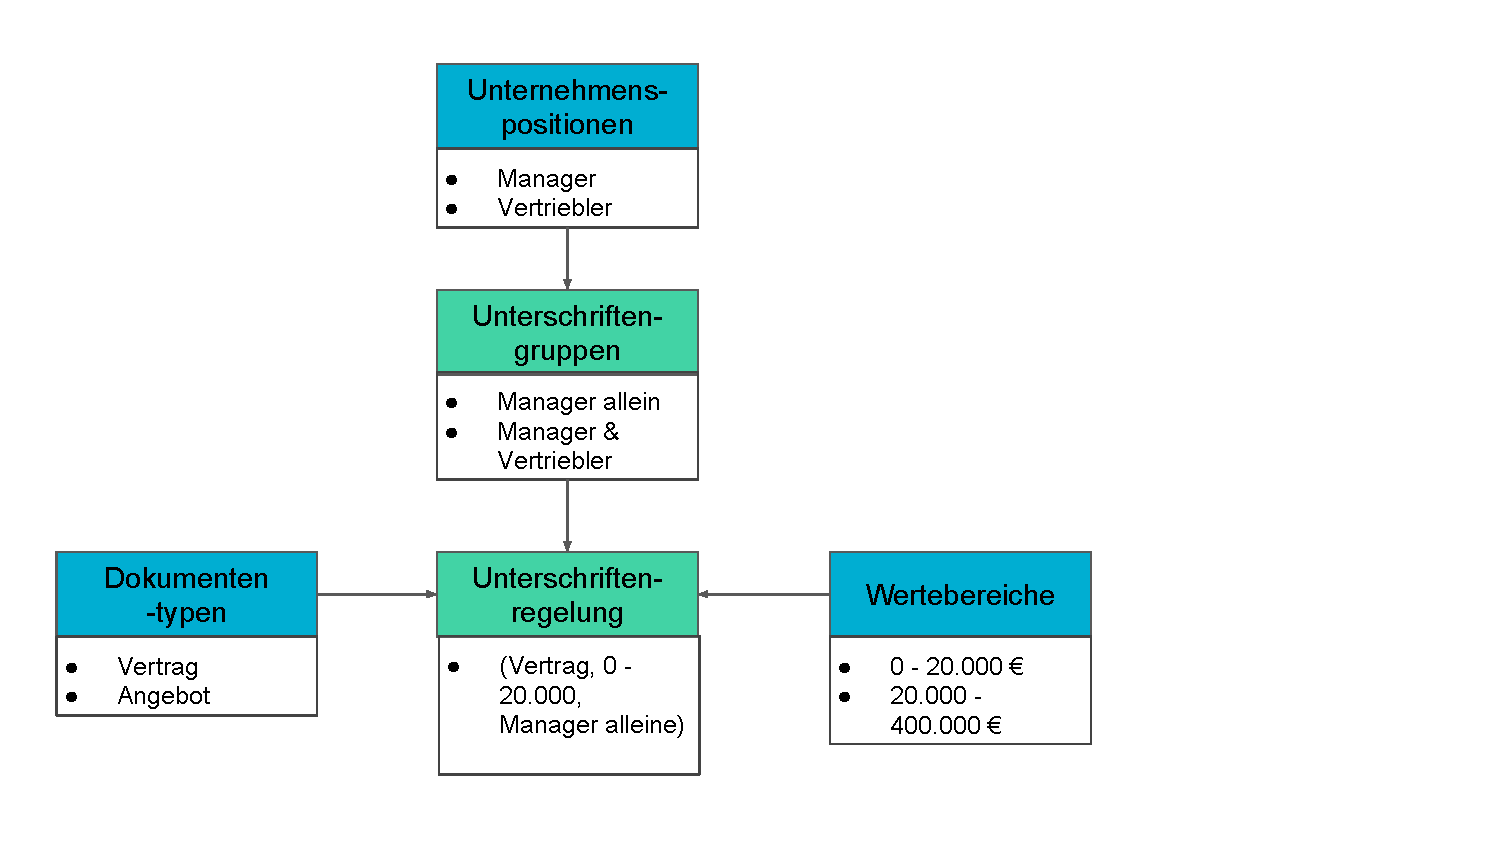
\includegraphics[width=0.8\textwidth, height=0.78\textheight]{./images/ruleSet}
	\end{figure}
\end{frame}

\begin{frame}{Problemlösung Detail}
	\begin{table}
		\begin{tabular}{|p{6cm}|p{6cm}|}\hline
			\rowcolor{codeBlue}\textbf{Problem} & \textbf{Lösung} \\ \hline
			\multirow{2}{*}{Zu hoher manueller Aufwand} & Elektronische Unterschreiben \\ \cline{2-2}
								& Automatisiertes Archivieren unterschriebener Dokumente \\ \hline
			\multirow{2}{*}{Falsch unterzeichnete Dokumente}  & Überprüfung ob Person unterschreiben darf \\ \cline{2-2}
								& Vorgabe der Unternehmenspositionsgruppen, die mit zu unterschreiben haben \\ \hline
		\end{tabular}
	\end{table}
\end{frame}

\begin{frame}{Ansatz Implementierung}
	\begin{itemize}
		\item Java \& Spring Boot
		\item RulesReader: SQL Datenbank
		\item UserReader: LDAP
		\item SigningConnector: DocuSign eSign
	\end{itemize}
	
\end{frame}


\section{Fazit}

\begin{frame}{Zusammenfassung}
	\begin{itemize}
		\item Im aktuellen Prozess sind Probleme vorhanden
		\item Verbesserungsvorschlag: Automatisierung \& Nutzung elektronischer Unterschrift
		\item Änderung der Rahmenbedingungen \& kurzer Zeitrahmen \newline $\Rrightarrow$ Keine Implementierung möglich
		\item Designvorschlag zur Umsetzung der Verbesserungsvorschläge
		\item Entwicklung der Datenstrukturen für den Prototypen
	\end{itemize}
\end{frame}	

\begin{frame}{Empfehlungen}
	\begin{itemize}
		\item Plugin für das ERP System vorhanden:
		\begin{itemize}
			\item Überprüfen ob das Tool die Bedingungen erfüllt
			\item Nutzung des Tools (Kosten-Nutzen Faktor besser)
		\end{itemize}
		\item Kein Plugin für das ERP System vorhanden:
		\begin{itemize}
			\item Recherche erneut kontrollieren
			\item System implementieren mit den empfohlenen Tools
			\item Überprüfung welche Daten benötigt werden (DSGVO konform)
		\end{itemize}
	\end{itemize}
\end{frame}

\vspace*{-15mm}   
\begin{frame}
	\begin{figure}
		\hspace*{-15mm}
		
\includegraphics[width=\paperwidth, height=\paperheight]{./images/questions.pdf}
	\end{figure}
\end{frame}

\end{document}
